\documentclass[a4paper,12pt]{article} % добавить leqno в [] для нумерации слева
\usepackage[a4paper,top=1.3cm,bottom=2cm,left=1.5cm,right=1.5cm,marginparwidth=0.75cm]{geometry}
%%% Работа с русским языком
\usepackage{cmap}					% поиск в PDF
\usepackage{mathtext} 				% русские буквы в фомулах
\usepackage[T2A]{fontenc}			% кодировка
\usepackage[utf8]{inputenc}			% кодировка исходного текста
\usepackage[english,russian]{babel}	% локализация и переносы

\usepackage{multirow}
\usepackage{graphicx}
\usepackage{mathtools}
\usepackage{wrapfig}
\usepackage{tabularx}
\usepackage{amssymb}
\usepackage{hyperref}
\usepackage[rgb]{xcolor}
\hypersetup{colorlinks=true,urlcolor=blue}
%% Шрифты
\usepackage{euscript}	 % Шрифт Евклид
\usepackage{amsmath}
\usepackage{mathtools}
%%% Заголовок
\author{Lokhmatov Arseniy}
\title{Лабораторная работа по общей физике}

\date{\today}
\begin{document}
\begin{titlepage}
    \newpage
    \begin{center}
    {\large МОСКОВСКИЙ ФИЗИКО-ТЕХНИЧЕСКИЙ ИНСТИТУТ (НАЦИОНАЛЬНЫЙ ИССЛЕДОВАТЕЛЬСКИЙ УНИВЕРСИТЕТ)}
    \vspace{1cm}

    {\largeФизтех-школа аэрокосмических технологий}
    \vspace{6em}
    \end{center}
    
    \vspace{1.2em}

    \begin{center}
    %\textsc{\textbf{}}
    \Large Лабораторная работа №4.4.4 \\
    Интерферометр Фабри-Перо
    \linebreak
    \end{center}
    
    \vspace{11em}
    
    \begin{flushright}
                       {\large Работу выполнил\\
                       Лохматов Арсений Игоревич\\
                       Б03-303 }
    \end{flushright}

    \vspace{\fill}

    \begin{center}
        
\includegraphics[width=0.2\linewidth]{dasr.png}
    \end{center}

    \begin{center}
    Долгопрудный, 2025
    \end{center}

    \end{titlepage}

\section{Теоретическая часть}

\paragraph{Цель работы:} измерение длины волны жлтых линий ртути, определение спектральных характеристик интерферометра Фабри-Перо.

\paragraph{Оборудование:} интерферометр Фабри-Перо, линзы, светофильтры, ртутная лампа, катетометр.

\begin{figure}[h]
\begin{center}
    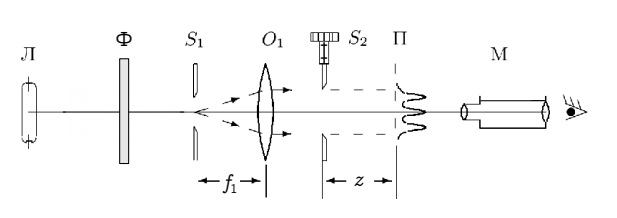
\includegraphics[width=16cm]{установка.png}
\end{center}
    \caption{Схема экспериментальной установки}
    \label{img1}
\end{figure}

\paragraph{Экспериментальная установка:} Схема экспериментальной установки приведеена на рисунке \ref{img1}. Свет от лампы $S$, пройдя через линзу $\text{Л}_0$ и светофильтр $\text{C}$, попадает ена интерферометр Фабри-Перо ($\text{ИФЛ}$). Линза $\text{Л}_0$ служит для формиравания пучка лучей (слегка сходящегося или слегка расходящегося). Интерференционные кольца наблюдаются в фокальной плоскости линзы $\text{Л}$. Картина рассматривается через зрительную трубу $\text{Т}$, сфокусированную на эту плоскость. Диаметр ыколец измеряются с помощью микроскопа катетометра. 

Зрительная труба $\text{Т}$, отсчётный микроскоп - элементы катетометра - прибора, предназначенного для измерения расстояний в вертикальной плоскости вдоль вертикальной оси.

При достаточной яркости лампы можно увидеть, что зелёная линия ртути состоит из нескольких компонентов. Расщепление этой спектральной линии связано с дополнительной энергией, возникающей как в результате взаимодействия магнитных моментов ядра и электрона - $\textit{сверхтонкая структура}$ (магнитное поле ядра действует на спиновый магнитный момент электрона), так и с $\textit{изотропическим сдвигом}$ (в парах ртути присутствуют в заметных количествах изотопы с атомными массами от 198 до 204 а.е.м) Каждое зелёное кольцо содержит более десятка близко расположенных компонентов, но разрешение нашего приборане позволяет всех их рассмотреть.

\section{Практическая часть}

\begin{enumerate}
    \item Включили ртутную лампу, оптическая система была отюстирована.
    \item Расположили в системе фильтр зелёного цвета. С помощью катетометра, систематическая погрешность которого примем за $\sigma_{\text{катет}} = 0.3 \text{ мм}$, измерим диаметра $5-6$ колец для спектральной линии. Для этого, монотонно перемещая зрительную трубу снизу вверх, определим координаты диаметров колец, начиная с самого дальнего от центра. Пройдя центр, последовательно определим вторые координаты тех же колец. В центре системы колец наблюдается яркий максимум, его мы исключили из нашего эксперимента. Поскольку кольца имеют определённую толщину, будем измерять расстояние до внутренней и до внешней окружностей, ограничивающих данное кольцо. Результаты измерений представлены в таблице $\ref{tab1}$.

    \[ d = \lvert d_1 - d_2\rvert \]

    \begin{table}[h]
        \centering
        \begin{tabular}{|c|c|c|c|c|c|c|c|}
        \hline
    	$N$ & $l_{\text{1 внутр}}, \text{ мм}$ & $l_{\text{1 внеш}}, \text{ мм}$ & $l_{\text{2 внутр}}, \text{ мм}$ & $l_{\text{2 внеш}}, \text{ мм}$ & $d_{\text{внутр}}, \text{ мм}$ & $d_{\text{внеш}}, \text{ мм}$ & $\overline{d}, \text{ мм}$ \\ \hline
    	1 & 183.865 & 184.044 & 146.205 & 145.912 & 37.660 & 38.132 & 37.896 \\ \hline
    	2 & 182.062 & 182.472 & 147.899 & 147.691 & 34.163 & 34.781 & 34.472 \\ \hline
    	3 & 180.109 & 180.731 & 149.871 & 149.559 & 30.238 & 31.172 & 30.705 \\ \hline
    	4 & 178.119 & 178.625 & 152.084 & 151.592 & 26.035 & 27.033 & 26.534 \\ \hline
    	5 & 176.159 & 175.334 & 154.636 & 154.075 & 20.698 & 22.084 & 21.391 \\ \hline
    	6 & 171.808 & 172.901 & 158.275 & 157.305 & 13.533 & 15.596 & 14.565 \\ \hline
        \end{tabular}
    \caption{Результаты измерений для фильтра зелёного цвета}
    \label{tab1}
    \end{table}

    \begin{table}[h]
        \centering
        \begin{tabular}{|c|c|c|c|}
        \hline
    	$N$ & $l_{\text{1}}, \text{ мм}$ & $l_{\text{2}}, \text{ мм}$ & $d, \text{ мм}$ \\ \hline
    	1 & 184.715 & 145.362 & 39.353 \\ \hline
    	2 & 184.101 & 145.859 & 38.242 \\ \hline
    	3 & 182.908 & 147.141 & 35.767 \\ \hline
    	4 & 182.322 & 147.742 & 34.580 \\ \hline
    	5 & 181.055 & 149.029 & 32.026 \\ \hline
    	6 & 180.379 & 149.655 & 30.724 \\ \hline
            7 & 178.939 & 151.208 & 27.731 \\ \hline
    	8 & 178.112 & 152.009 & 26.103 \\ \hline
    	9 & 176.485 & 153.735 & 22.750 \\ \hline
    	10 & 175.491 & 154.781 & 20.710 \\ \hline
    	11 & 172.659 - 173.761 & 156.568 - 157.429 & 15.230 - 17.193 \\ \hline
    	12 & 171.189 - 172.259 & 157.966 - 158.985 & 12.204 - 14.293 \\ \hline
        \end{tabular}
    \caption{Результаты измерений для фильтра жёлтого цвета}
    \label{tab2}
    \end{table}

    \item Для оценки $\textit{аппаратной}$ разрешающей способности (характеристики установки в целом), измерим ширину $\delta r$ колец. Результаты вычислений рапишем в таблицу $\ref{tab3}$.

    \[ \delta r = \lvert r_{\text{внутр}} - r_{\text{внеш}}\rvert \]

    \begin{table}[h]
        \centering
        \begin{tabular}{|c|c|c|c|c|c|c|}
        \hline
            \multicolumn{4}{|c|}{\text{Зелёный фильтр}} \\ \hline
        \hline
    	$N$ & $\delta r_1, \text{ мм}$ & $\delta r_2, \text{ мм}$ & $\overline{\delta r}, \text{ мм}$ \\ \hline
    	1 & 0.179 & 0.293 & 0.236 \\ \hline
    	2 & 0.410 & 0.208 & 0.309 \\ \hline
    	3 & 0.622 & 0.312 & 0.467 \\ \hline
    	4 & 0.506 & 0.492 & 0.499 \\ \hline
    	5 & 0.825 & 0.561 & 0.693 \\ \hline
    	6 & 1.093 & 0.970 & 1.032 \\ \hline
        \end{tabular}
        \begin{tabular}{|c|c|c|c|c|c|c|}
        \hline
            \multicolumn{3}{|c|}{\text{Жёлтый фильтр}} \\ \hline
        \hline
    	$N$ & $\delta r, \text{ мм}$ & $\overline{\delta r}, \text{ мм}$ \\ \hline
    	11 & 0.861 - 1.102 & 0.981 \\ \hline
    	12 & 1.019 - 1.070 & 1.044 \\ \hline
        \end{tabular}
    \caption{Результаты измерений для различных фильтров}
    \label{tab3}
    \end{table}

    Так же запишем параметры установки: фокусное расстояние линзы $\text{Л}$ составляет (фокусное расстояние этой линзы мы измеряли самостоятельно с помощью экрана и линейки с систематической погрешностью $\sigma_{f} = 1 \text{ мм}$) $f = (120 \pm 1) \text{ мм}$ и расстояние между зеркалами интерферометра (база интерферометра) $L = 0.1 \text{ мм}$.

    \item Оценим
    \begin{enumerate}
        \item максимальный порядок интерференции $m$ (номер центрального кольца) для зелёной линии ртути по формуле

        \[ 2L\cos{\Theta_m} = m\lambda, \text{ где } r = d / 2, \text{ } \cos{\Theta_m} = \frac{f}{\sqrt{f^2+r^2}}. \]

        где $\Theta_m$ - угол падения волны, длина которой $\lambda$. Полагаем, что $\lambda_{\text{зел}} = 56\cdot10^{-5} \text{ мм} $, $\lambda_{\text{жел}} = 58\cdot10^{-5} \text{ мм} $, тогда

        \[ m = \biggl[\frac{2L\cos{\Theta_m}}{\lambda}\bigg] - \text{целое число}.\]

        Результаты вычислений представлены в таблице $\ref{tab4}$ для зелёной линии ртути и в таблице $\ref{tab5}$ для жёлтой линии ртути.

    \begin{table}[h]
        \centering
        \begin{tabular}{|c|c|c|c|c|c|c|}
        \hline
    	$N$ & $r_1, \text{ мм}$ & $r_2, \text{ мм}$ & $\overline{r}, \text{ мм}$ & $\cos{\Theta_m}$ & m & $\Delta\lambda, \text{ } \mathring A$ \\ \hline
    	1 & 18.830 & 19.066 & 18.948 & 0.988 & 353 & 15.864 \\ \hline
    	2 & 17.082 & 17.391 & 17.236 & 0.990 & 354 & 15.819 \\ \hline
    	3 & 15.119 & 15.586 & 15.353 & 0.992 & 355 & 15.775 \\ \hline
    	4 & 13.018 & 13.517 & 13.267 & 0.994 & 356 & 15.730 \\ \hline
    	5 & 10.349 & 11.042 & 10.696 & 0.996 & 356 & 15.730 \\ \hline
    	6 & 6.766 & 7.798 & 7.282 & 0.998 & 357 & 15.686 \\ \hline
        \end{tabular}
    \caption{Результаты вычислений для фильтра зелёного цвета}
    \label{tab4}
    \end{table}

    Видим, что максимальный порядок интерференции для зелёной линии ртути достигается в самом близком к центру кольцу и равен $m = 357$.

    \begin{table}[h]
        \centering
        \begin{tabular}{|c|c|c|c|c|c|c|}
        \hline
    	$N$ & $r, \text{ мм}$ & $\cos{\Theta_m}$ & m & $\Delta\lambda, \text{ } \mathring A$ \\ \hline
    	1 & 19.676 & 0.987 & 340 & 17.059 \\ \hline
    	2 & 19.121 & 0.988 & 340 & 17.059 \\ \hline
    	3 & 17.883 & 0.989 & 341 & 17.009 \\ \hline
    	4 & 17.290 & 0.990 & 341 & 17.009 \\ \hline
    	5 & 16.013 & 0.991 & 342 & 16.959 \\ \hline
    	6 & 15.362 & 0.992 & 342 & 16.959 \\ \hline
        \end{tabular}
        \begin{tabular}{|c|c|c|c|c|c|c|}
        \hline
    	$N$ & $r, \text{ мм}$ & $\cos{\Theta_m}$ & m & $\Delta\lambda, \text{ } \mathring A$ \\ \hline
    	7 & 13.865 & 0.993 & 342 & 16.959 \\ \hline
    	8 & 13.051 & 0.994 & 342 & 16.959 \\ \hline
    	9 & 11.375 & 0.996 & 343 & 16.960 \\ \hline
    	10 & 10.355 & 0.996 & 343 & 16.960 \\ \hline
    	11 & 8.106 & 0.998 & 344 & 16.860 \\ \hline
    	12 & 6.624 & 0.998 & 344 & 16.860 \\ \hline
        \end{tabular}
    \caption{Результаты вычислений для фильтра жёлтого цвета}
    \label{tab5}
    \end{table}

    Видим, что максимальный порядок интерференции для жёлтой линии ртути достигается в самом близком к центру кольцу и равен $m = 344$.

    \item дисперсионную область $\Delta\lambda$ по формуле:

    \[ m(\lambda + \Delta\lambda) = (m+1)\lambda \Longleftrightarrow \Delta\lambda = \frac{\lambda}{m}. \]
    
    Результаты вычислений представлены в таблице $\ref{tab4}$ для зелёной линии ртути и в таблице $\ref{tab5}$ для жёлтой линии ртути.
    \end{enumerate}

    \item Построим график $d^2_i=F(i)$ для зелёной линии ртути, приняв $\lambda(Hg)=5461 \text{ } \mathring A$. Результат представлен на рисунке $\ref{img2}$.

    \begin{figure}[h]
    \begin{center}
        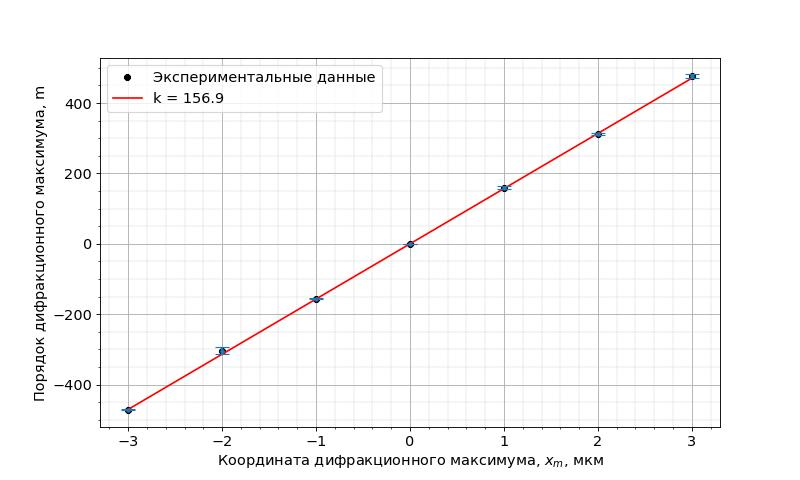
\includegraphics[width=16cm]{image1.jpg}
    \end{center}
        \caption{График зависимости функции $d^2_i=F(i)$}
        \label{img2}
    \end{figure}

    Диаметр интерференционного кольца $d$ и угол падения световой волны $\theta$ для малых $\theta$ связаны соотношением $\theta=\frac{d}{2f}$, где $f$ - фокусное расстояние линзы $\text{Л}$.

    Для малых углов $\theta$ для условия возникновения интерференционного кольца верно следующее преобразование:

    \[ \Delta = 2L\Bigl(\frac{1}{\cos{\theta}} -\tan{\theta}\sin{\theta} \Bigr)=2L\cos{\theta} \Longleftrightarrow \theta^2_m = 2-\frac{\lambda}{L}m. \]

    При переходе от любого кольца к соседнему с большим диаметром порядок интерференции уменьшается на 1. Так как кольца пронумерованы $i=1\rightarrow6$, возникает зависимость угла на максимума интерференции от его номера или диаметра кольца:

    \[ \frac{d^2(i)}{4f^2}=\theta^2(i)=const + \frac{\lambda}{L}i \Longleftrightarrow d^2(i) = 4f^2\frac{\lambda}{L}i+const'. \]

    Из этого следует, что есть экспериментальную зависимость аппроксимировать прямой, то, зная коэффициент наклона этой прямой, можно найти базу интерферометра $L$ (знак минус показывает, что зависимость уменьшается).

    \[ 4f^2\frac{\lambda}{L} = |k|=244.309 \Longleftrightarrow L = \frac{4f^2\lambda}{|k|} \Longrightarrow L = \frac{4\cdot120^2\cdot5461\cdot10^{-10}}{244.309} = 0.129 \text{ мм} \approx 0.1 \text{ мм}, \]

    то есть значение базы интерферометра, указанное на установке, совпадает со значением, полученным экспериментально с учётом погрешности.

    \item Рассчитаем средние диаметры $\overline{d}$ для жёлтых пар колец $Hg$ и разности диаметров $\Delta d$ для колец одного порядка. Результаты вычислений представлены в таблице $\ref{tab6}$.

    \begin{table}[h]
        \centering
        \begin{tabular}{|c|c|c|c|c|}
        \hline
    	$N$ & $d, \text{ мм}$ & $\overline{d}, \text{ мм}$ & $\Delta d, \text{ мм}$ \\ \hline
    	1 & 39.353 & \multirow{2}{*}{38.798} & \multirow{2}{*}{1.111} \\
    	2 & 38.242 & & \\ \hline
    	3 & 35.767 & \multirow{2}{*}{35.174} & \multirow{2}{*}{1.187} \\
    	4 & 34.580 & & \\ \hline
    	5 & 32.026 & \multirow{2}{*}{31.375} & \multirow{2}{*}{1.302} \\
    	6 & 30.724 & & \\ \hline
        \end{tabular}
        \begin{tabular}{|c|c|c|c|}
        \hline
    	$N$ & $d, \text{ мм}$ & $\overline{d}, \text{ мм}$ & $\Delta d, \text{ мм}$ \\ \hline
    	7 & 27.731 & \multirow{2}{*}{26.917} & \multirow{2}{*}{1.628} \\
    	8 & 26.103 & & \\ \hline
    	9 & 22.750 & \multirow{2}{*}{21.730} & \multirow{2}{*}{2.040} \\
    	10 & 20.710 & & \\ \hline
    	11 & 16.212 & \multirow{2}{*}{14.730} & \multirow{2}{*}{2.964} \\
    	12 & 13.248 & & \\ \hline
        \end{tabular}
    \caption{Результаты вычислений для фильтра жёлтого цвета}
    \label{tab6}
    \end{table}

    Построим график $\overline{d}=F(1/\Delta d)$. Результат представлен на рисунке $\ref{img3}$.

    \begin{figure}[h]
    \begin{center}
        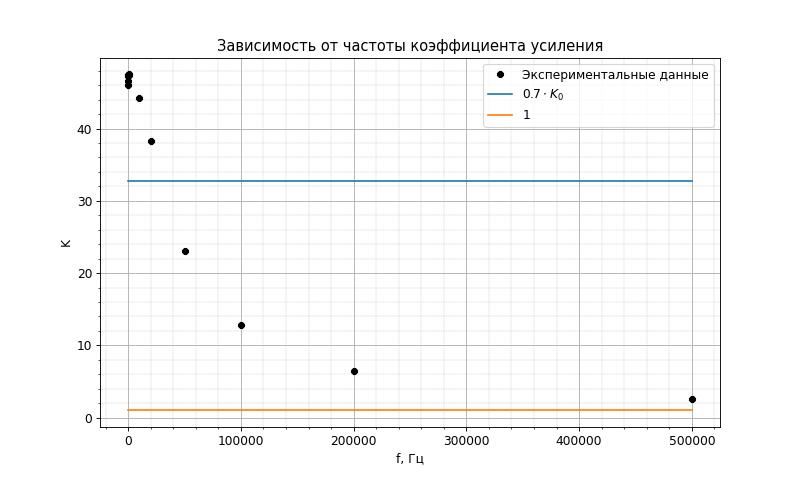
\includegraphics[width=16cm]{image2.jpg}
    \end{center}
        \caption{График зависимости функции $\overline{d}=F(1/\Delta d)$}
        \label{img3}
    \end{figure}

    По углу наклона получившейся прямой рассчитаем разность длин волн $\Delta \lambda$ для жёлтой пары линий ртути $\bigl[\overline{\lambda}=5780 \mathring A\bigr]$, используя формулу:

    \[ \Delta \lambda = \lambda\Theta\Delta\Theta=\frac{\lambda\overline{d}\Delta d}{4f^2} \Longleftrightarrow \overline{d}=\frac{4f^2\Delta\lambda}{\lambda}\frac{1}{\Delta d} \]

    \[ \frac{4f^2\Delta\lambda}{\lambda} = k = 40.665 \text{ мм}^2 \Longleftrightarrow \Delta\lambda=\frac{\lambda k}{4f^2} \Longrightarrow \Delta\lambda=\frac{5780\cdot10^{-7}\cdot40.665}{4\cdot120^2} = 4.081\text{ }\mathring A. \]

    \item Оценим экспериментальное значение линейной дисперсии интерферометра, использу разность диаметров и разность длин волн жёлтых пар полец ртути и сравним с теоретическим значением по формулам:

    \[ D^*_{\text{эксп}} = f\frac{d\theta}{d\lambda}=\frac{\Delta d}{2\cdot\Delta\lambda}, \text{ } D^*_{\text{эксп}} = \frac{2f^2}{\lambda\cdot d}. \]

    Результаты вычислений представлены в таблице $\ref{tab7}$.

    \begin{table}[h]
        \centering
        \begin{tabular}{|c|c|c|c|}
        \hline
    	$N$ & $D^*_{\text{эксп}}, \text{ мм/}\mathring A$ & $D^*_{\text{теор}}, \text{ мм/}\mathring A$ & $\overline D^*_{\text{теор}}, \text{ мм/}\mathring A$ \\ \hline
    	1 & \multirow{2}{*}{0.136} & 0.127 & \multirow{2}{*}{0.128} \\
    	2 &  & 0.130 & \\ \hline
    	3 & \multirow{2}{*}{0.145} & 0.139 & \multirow{2}{*}{0.142} \\
    	4 &  & 0.144 & \\ \hline
    	5 & \multirow{2}{*}{0.160} & 0.156 & \multirow{2}{*}{0.159} \\
    	6 &  & 0.162 & \\ \hline
    	7 & \multirow{2}{*}{0.199} & 0.180 & \multirow{2}{*}{0.185} \\
    	8 &  & 0.191 & \\ \hline
    	9 & \multirow{2}{*}{0.250} & 0.219 & \multirow{2}{*}{0.230} \\
    	10 &  & 0.241 & \\ \hline
    	11 & \multirow{2}{*}{0.363} & 0.307 & \multirow{2}{*}{0.342} \\
    	12 &  & 0.376 & \\ \hline
        \end{tabular}
    \caption{Результаты вычислений для фильтра жёлтого цвета}
    \label{tab7}
    \end{table}

    Видим, что порядок значений совпадает.

    \newpage

    \item Оценим аппаратную разрешающую способность, рассчитав $\delta\lambda$ через диаметр кольца $d$ и его ширину $\delta r$.

    \[ 2L\cos{\Theta}=m\lambda \longrightarrow \text{(дифференцируем)} \longrightarrow \] \[ \longrightarrow -2L\sin{\Theta}\delta\Theta =m\delta\lambda \longrightarrow \text{(делим одно на другое по модулю)} \longrightarrow \] \[ \longrightarrow R_{\text{апп}} = \frac{\delta\lambda}{\lambda} = \frac{\cos{\Theta}}{\sin{\Theta}\delta\Theta} \simeq \frac{1}{\Theta\cdot\delta\Theta} \simeq \frac{4f^2}{d\cdot\delta r}. \]

    Оценим число интерферирующих лучей по аналогии с решёткой по формуле $R_{\text{апп}}=m\cdot N$.

    А так же рассчитаем теоретические значения добротности интерферометров по формуле:

    \[ R_{\text{апп}}^{\text{теор}} = \frac{\lambda}{\delta\lambda} = \frac{\pi\sqrt{r}}{1-r}m, \text{ где $r\simeq0.85$ - коэффициент отражения}.  \]

    Так же оценим теоретическое значение числа интерферирующих лучей. Результаты вычислений преведены в таблице \ref{tab8}.

    \begin{table}[h]
        \centering
        \begin{tabular}{|c|c|c|c|c|}
        \hline
            \multicolumn{5}{|c|}{\text{Зелёный фильтр}} \\ \hline
        \hline
    	$N$ & $R_{\text{апп}}$ & $N_{\text{инт.луч.}}$ & $R_{\text{апп}}^{\text{теор}}$ & $N_{\text{инт.луч.}}^{\text{теор}}$ \\ \hline
            1 & 6440.463 & 18 & 6816.207 & 19 \\ \hline
    	2 & 5407.512 & 15 & 6835.517 & 19 \\ \hline
            3 & 4016.951 & 11 & 6854.826 & 19 \\ \hline
    	4 & 4350.300 & 12 & 6874.135 & 19 \\ \hline
    	5 & 3885.601 & 10 & 6874.135 & 19 \\ \hline
    	6 & 3832.060 & 10 & 6893.445 & 19 \\ \hline
        \end{tabular}
        \begin{tabular}{|c|c|c|c|c|}
        \hline
            \multicolumn{5}{|c|}{\text{Жёлтый фильтр}} \\ \hline
        \hline
    	$N$ & $R_{\text{апп}}$ & $N_{\text{инт.луч.}}$ & $R_{\text{апп}}^{\text{теор}}$ & $N_{\text{инт.луч.}}^{\text{теор}}$ \\ \hline
    	11 & 3621.960 & 10 & 6642.423 & 19 \\ \hline
    	12 & 4164.584 & 12 & 6642.423 & 19 \\ \hline
        \end{tabular}
    \caption{Результаты измерений для различных фильтров}
    \label{tab8}
    \end{table}

    Видим, что значения, полученные в ходе эксперимента, совпадают с теоретическими значениями с учётом погрешности при рассмотрении дальних колец. Такой результат, предположительно, связан с тем, что интерферометр был настроен не на центр колец, а на их дуги.

\end{enumerate}
    
    \newpage

    \section{Вывод}

    В ходе работы мы измеряли спектральные характеристики интерферометра Фабри-Пето в случае наблюдения натриевой лампы.

    Мы определили Линейную дисперсию $D$ интерферометра, сравнили его с теоретическим. Значения достаточно близки друг к другу и совпадают с учётом погрешности.

    Мы измерили дисперсионную область интерферометра $\Delta\lambda$. Результат согласуется с действительностью, потому что интерферометр Фабри-Перо имеет достаточно большую аппаратную разрешающую способность, но он использовался для анализа довольно узких спектров.

    Была определена аппаратная разрешающая способность $R_{\text{апп}}$ интерферометра и число интерферирующих лучей. Полученные значения совпадают с теоретическими по порядку величины и в частных случаях.

\end{document}
